%----------------------------------------------------------------------------
\chapter{A generált monitor forráskód helyességének tesztelése}
%----------------------------------------------------------------------------

%----------------------------------------------------------------------------
\section{Tesztelési célok}
%----------------------------------------------------------------------------

A generált monitor forráskód tesztelésére a következő célokat fogalmazuk meg:

\begin{itemize}
    \item Az összes üzenet típus megjelenése a különböző teszt szcenáriókban
    \item Időzített feltételek helyes kiértékelése
    \item Üzenet megkötések tesztelése
    \item \textit{Alt} és \textit{Par} operátorok esetén, az üzenet szekvencia ágak helyes kiértékelése
    \item \textit{Loop} operátor esetén a minimális és maximálás üzenet ismétlődések tesztelése
    \item Összetett szcenárió tesztelése, ami több operátort tartalmaz
    \item Egymást követő elvárt üzeneteket tartalmazó szcenárió tesztelése
    \item Egymást követő \textit{fail} üzeneteket tartalmazó szcenárió tesztelése
    \item \textit{Regular} üzenet tesztelése (ha megjelenik a rendszer működésében akkor ki kell értékelni a szenárió többi részét, ha nem jelenik meg a monitor helyes működést kell jelezzen és, hogy a követelmény nem teljesült)
    \item Több óraváltozót tartalmazó szcenárió tesztelése
    \item Egymást követő üzenetek kombinációinak tesztelése (pl. elvárt üzenetet követő \textit{fail}, elvárt üzenetet követő reguláris, stb.)
\end{itemize}

%----------------------------------------------------------------------------
\clearpage\section{Monitor forráskód generátor tesztelése}
%----------------------------------------------------------------------------

A generált monitor forráskodját integrációs tesztek segítségével szeretnénk ellenőrizni.
Az \textit{Xtext} keretrendszer a specifikált \textit{DSL (Domain Specific Language)} nyelvhez generál egy \textit{Maven} \textit{plugin}-t.
Ezt a \textit{plugin}-t betölthetjük egy egyszerű \textit{Maven} projektbe és használhatjuk is az elkészített \textit{DSL} nyelvünket, azaz létrehozhatunk a projektben a saját \textit{DSL}-ünkhöz tartozó fájlokat, melyekben megadhatjuk saját szcenárióinkat.

\begin{figure}[!ht]
    \centering
    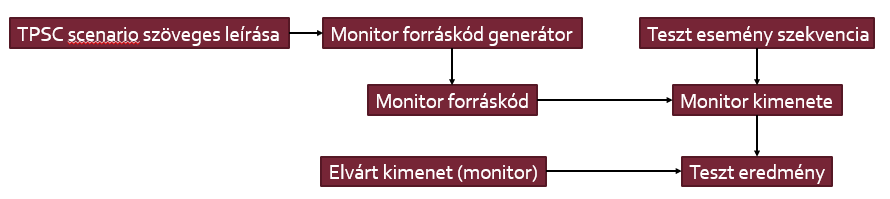
\includegraphics[width=150mm, height=9cm, keepaspectratio]{figures/integration_test_flow.png}
    \caption{Integrációs tesztelés folyamatábrája.}
    \label{testing_figure}
\end{figure}

A \ref{testing_figure} ábrán megtekinthető az integrációs tesztelés tervének folyamatábrája.

Egy integrációs teszt akkor sikeres ha a monitor kimenete megegyezik az elvárt kimenettel.

%----------------------------------------------------------------------------
\clearpage
%----------------------------------------------------------------------------

Az \textit{Xtext} keretrendszer által nyujtott \textit{Maven plugin}-t felhasználhatjuk az integrációs teszteinkhez.
Elég csupán egy \textit{Maven} projektet felkonfigurálni a saját \textit{DSL plugin}-ünkkel és elkészítethetjük a saját tesztelési keretrendszerünket.
Ezek a \textit{Maven} projektek a szülő projektünkben helyezkedhetnek el, így a projekt struktúrában közvetlen a nyelvünk mellett vannak.
A \ref{integration_test_structure} ábrán  kódrészléten látható egy ilyen integrációs teszthez tartozó \textit{Maven} projekt felépítése

\begin{figure}[!ht]
    \centering
    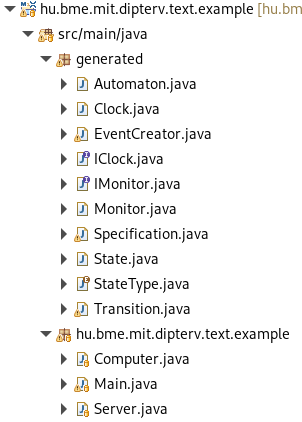
\includegraphics[width=150mm, height=9cm, keepaspectratio]{figures/integration_test_structure.png}
    \caption{Példa integrációs teszt projekt struktúrája.}
    \label{integration_test_structure}
\end{figure}

A \ref{integration_test_structure} ábrán lévő \textit{generated} csomag tartalmazza a szcenárióhoz tartozó generált automata forráskódját és a monitor forráskódját.

\begin{lstlisting}[language=java, frame=single, float=ht!, caption={Integrációs teszteset eredménye.},captionpos=b,label=maven_test_output]
-------------------------------------------------------
T E S T S
-------------------------------------------------------
Running hu.bme.mit.dipterv.text.example.MonitorPassingTest
q0 NORMAL
q1 NORMAL
q2 ACCEPT
q3 NORMAL
q4 NORMAL
q5 FINAL
!(computer.checkEmail().computer) q0->q0
computer.checkEmail().computer q0->q1
!(computer.sendUnsentEmail().server) q1->q1
!(computer.sendUnsentEmail().server) q1->q2
computer.sendUnsentEmail().server q1->q3
!(computer.logout().server) & !(computer.newEmail().server) q3->q3
computer.newEmail().server q3->q4
!(computer.downloadEmail().server) q4->q4
computer.downloadEmail().server q4->q5
Received Message: computer.checkEmail().computer
Transition: !(computer.checkEmail().computer)
Transition: computer.checkEmail().computer
transition triggered: computer.checkEmail().computer
q1

Received Message: computer.sendUnsentEmail().server
Transition: !(computer.sendUnsentEmail().server)
Transition: !(computer.sendUnsentEmail().server)
Transition: computer.sendUnsentEmail().server
transition triggered: computer.sendUnsentEmail().server
q3

Received Message: computer.newEmail().server
Transition: !(computer.logout().server) & !(computer.newEmail().server)
Transition: computer.newEmail().server
transition triggered: computer.newEmail().server
q4

Received Message: computer.downloadEmail().server
Transition: !(computer.downloadEmail().server)
Transition: computer.downloadEmail().server
transition triggered: computer.downloadEmail().server
q5

Tests run: 1, Failures: 0, Errors: 0, Skipped: 0, Time elapsed: 0.025 sec

Results :

Tests run: 1, Failures: 0, Errors: 0, Skipped: 0
\end{lstlisting}

A \ref{maven_test_output} kódrészlet a \textit{Maven} teszt kimenetét tartalmazza.

Ezt a projekt struktúrát felhasználva a teszteink köré tudunk egy \textit{Maven} alapú \textit{Continuous Integration}-t (\textit{CI}) állítani a generált monitor forráskód folyamatos ellenőrzése érdekében.

%----------------------------------------------------------------------------
\clearpage\section{Continuous Integration}\subsection{Github Actions CI}
%----------------------------------------------------------------------------

Az időzített automata és monitor forráskód generátorok automatikus tesztelése a \textit{Github Actions} segítségével történik.
A \textit{CI} minden feltöltött új commit esetén lefut.
A \textit{CI} különböző fázisai a következők:

\begin{itemize}
    \item I. Teljes \textit{Xtext} projekt fordítása (\textit{Maven})
    \item II. Intergrációs tesztek futtatása
\end{itemize}

A generátorokhoz tartozó \textit{Xtext} projekten lefut egy \textit{Maven build}, amely az új feltöltött verzió tartalmazza.
Ez a \textit{build} állítja elő a \textit{DSL} nyelvhez tartozó \textit{Maven plugin}-t is.
Ezt követően hajtódnak végre az integrációs tesztek, amelyek a frissen fordított \textit{Maven plugin}-t használják.
Ha az összes fázis sikeresen lefutott, akkor az adott változtatás nem rontott el semmilyen korábbi funkciót.
A \textit{CI}-hoz tartozó \textit{script}-et a \ref{ci_script} kódrészlet tartalmazza.

\begin{figure}[!ht]
    \centering
    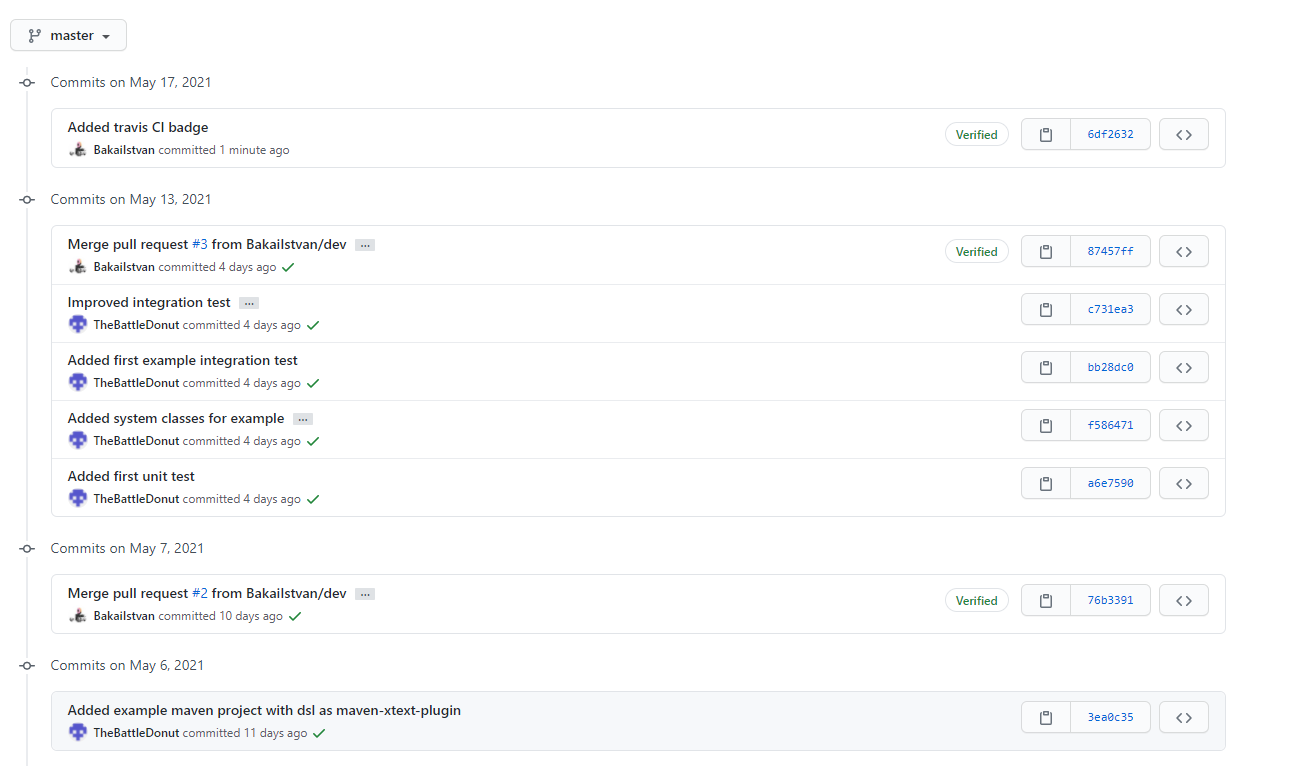
\includegraphics[width=150mm, keepaspectratio]{figures/github_ci_check.png}
    \caption{GitHub repository commit-ok és hozzá tartozó CI check-ek.}
\end{figure}

\begin{figure}[!ht]
    \centering
    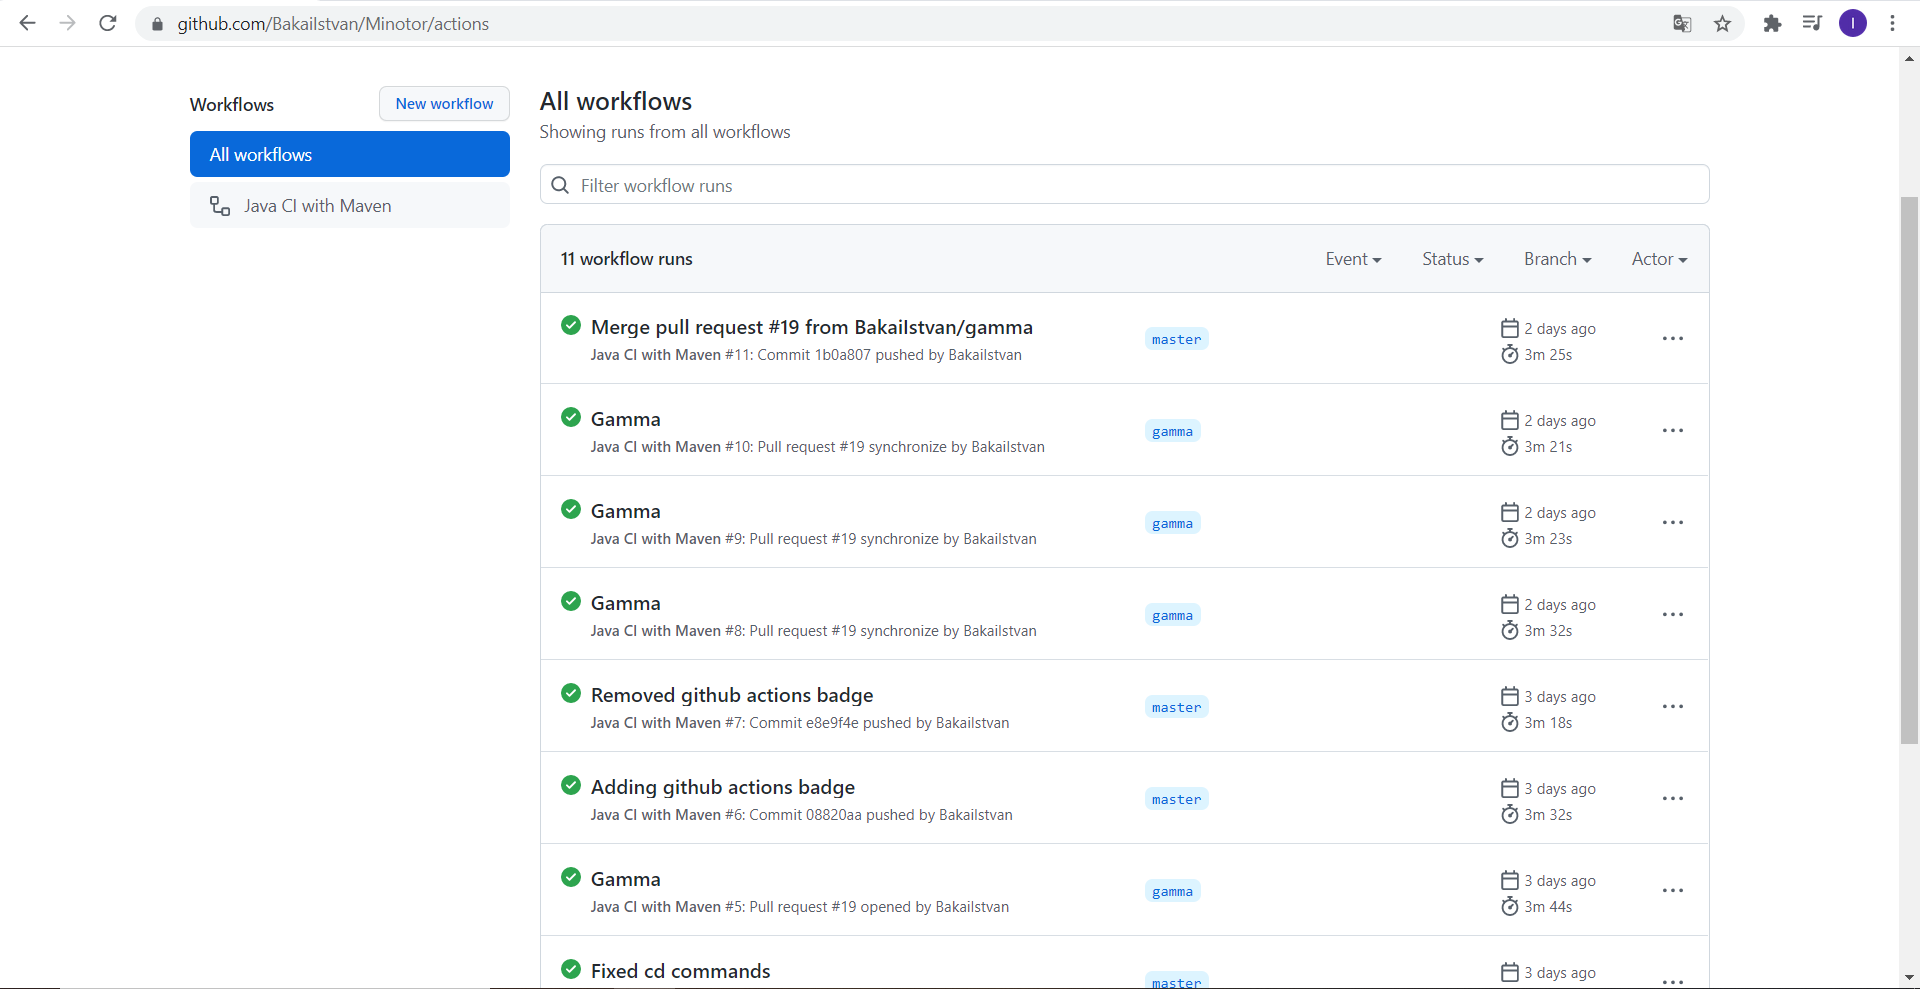
\includegraphics[width=150mm, keepaspectratio]{figures/github_ci_builds.png}
    \caption{Github Actions CI build-ek eredményei.}
\end{figure}

\begin{lstlisting}[language=java, frame=single, float=ht!, caption={Github Actions CI-hoz tartozó .yml script.},captionpos=b,label=ci_script]
# This workflow will build a Java project with Maven, and cache/restore any dependencies to improve the workflow execution time
# For more information see: https://help.github.com/actions/language-and-framework-guides/building-and-testing-java-with-maven

name: Java CI with Maven

on:
    push:
    branches: [ master ]
    pull_request:
    branches: [ master ]

jobs:
    build:

    runs-on: ubuntu-latest

    steps:
    - uses: actions/checkout@v2
    - name: Set up JDK 11
        uses: actions/setup-java@v2
        with:
        java-version: '11'
        distribution: 'adopt'
        cache: maven
    - name: Build with Maven
        run: mvn clean install -U
    - name: Test example project
        run: cd hu.bme.mit.dipterv.text.example; mvn clean install -U
    - name: Test mobileexample project
        run: cd hu.bme.mit.dipterv.text.mobileexample; mvn clean install -U
    - name: Test altexample project
        run: cd hu.bme.mit.dipterv.text.altexample; mvn clean install -U
    - name: Test parexample project
        run: cd hu.bme.mit.dipterv.text.parexample; mvn clean install -U
    - name: Test operatorexample project
        run: cd hu.bme.mit.dipterv.text.operatorexample; mvn clean install -U
    - name: Test gamma integration project
        run: cd hu.bme.mit.dipterv.text.gammaexample; mvn clean install -U
\end{lstlisting}

%----------------------------------------------------------------------------
\clearpage\section{Tesztesetek}\subsection{Egyszerű időzítési megkötéseket tartalmazó tesztszenárió}
%----------------------------------------------------------------------------

A tesztesetekhez tartozó scenario követelmény megtalálható az \ref{example_test_scenario} kódrészleten.
A szcenárióhoz tartozó diagram a \ref{example_test_scenario_diagram} ábrán látható

\begin{lstlisting}[language=java, frame=single, float=ht!, caption={Integrációs tesztesethez tartozó szcenárió szöveges leírása.},captionpos=b,label=example_test_scenario]
specification Email {

	object Computer computer;
	object Server server;

	integer timeout = 10;
	string receiver = "John";
	string subject = "Next meeting";

	clock x;

	constraint constraints {
		message logout() computer -> server;
	}

	scenario sendEmail{
		message checkEmail() computer -> computer reset x;
		required message sendUnsentEmail() computer -> server;
		pastConstraint {constraints} message newEmail(receiver, subject) computer -> server;
		message downloadEmail(timeout) computer -> server clockConstraint {>(x,10)};
	}
}
\end{lstlisting}

\begin{figure}[!ht]
    \centering
    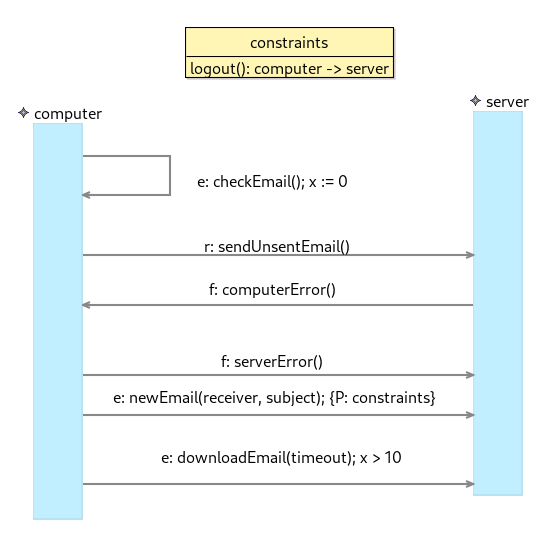
\includegraphics[width=150mm, keepaspectratio]{figures/diagramExample.png}
    \caption{Szcenárió diagram vizualízációja.}
    \label{example_test_scenario_diagram}
\end{figure}

A rendszer egy szervergépből és egy felhasználói számitogépből áll.
A szerver egy \textit{e-mail} szervert szimulál, aminek a számitogép különböző kéréseket küldhet.
Például lekérdezheti tőle a kapott \textit{e-mail} vagy új \textit{e-mail} küldhet.
A követelményben leírjuk, hogy a rendszernek mi a helyes viselkedése \textit{e-mail} küldés esetén.
Ha a computer a \textit{checkEmail} hívást használva talál elküldendő \textit{e-mail} az továbbítja a szervernek.
Ezt az \textit{elvárt} \textit{sendUnsentEmail} üzenet jelzi.
Ezt követően meg kell jelenjen a rendszer működésében a \textit{newEmail} üzenet.
Ha ehelyett \textit{logout} üzenet érkezik a hibás működést jelent.
A \textit{newEmail} üzenetet a \textit{downloadEmail} üzenet követi.
Ezen az üzeneten van egy 10 másodperces időzítési feltétel, ami a letöltést szimulálja.

A szcenárióhoz tartozó tesztesetek a következők:

\begin{itemize}
    \item testNetworkRequirementSatisfied
    \item testNetworkNoErrors
    \item testNetworkWithErrors
    \item testNetworkWithNoDelay
    \item testNetworkFirstFail
    \item testNetworkSecondFail
\end{itemize}

A \textit{testNetworkRequirementSatisfied} tesztesetben a rendszer helyes működését szimuláljuk és azt ellenőrizzük, hogy a generált monitor képes ezt érzékelni és jelzi.
A \textit{testNetworkNoErrors} azt vizsgálja, hogy a monitor képes-e érzékelni, hogy a rendszer nem felelt meg a követelménynek.
Itt úgy manipuláljuk a teszt rendszer, hogy lehagyjuk a letöltés részt a működésből.
Ilyenkor a rendszer nem felel meg a követelménynek, viszont még jó állapotban marad, mert nem történt hiba.
A \textit{testNetworkWithErrors} tesztesetnél a \textit{sendUnsentEmail} üzenet után egy \textit{logout} üzenetet küldünk a monitor és azt vizsgáljuk képes-e detektálni ezt a hibát.
A \textit{testNetworkWithNoDelay}-nél pedig túl gyorsan küldjük a működés végén a \textit{downloadEmail} üzenetet és azt ellenőrizzük képes e a monitor ezt a hibát érzékelni.

%----------------------------------------------------------------------------
\clearpage\subsection{Többféle üzenetet és megkötést tartalmazó egyszerű tesztszenárió}
%----------------------------------------------------------------------------

\begin{lstlisting}[language=java, frame=single, float=ht!, caption={Második tesztesethez tartozó szcenárió.},captionpos=b,label=second_scenario_test]
    specification Photo{

        object User user;
        object Device device;
        object Database db;

        clock x;

        constraint error {
            message closeApp() user -> device;
        }

        scenario playlist_generation{
            message openApp() user -> device reset x;
            message accessWebcam() device -> device clockConstraint {<=(x, 5)} reset x;
            required futureConstraint {error} message getPhoto() device -> user;
            fail message cameraOffline() user -> device;
            required strict message retrieveMood() device -> db;
            required message retrieveMusic() device -> db;
            strict message generatePlaylist() db -> device clockConstraint {<(x, 15)};
        }
    }
\end{lstlisting}

\begin{figure}[!ht]
    \centering
    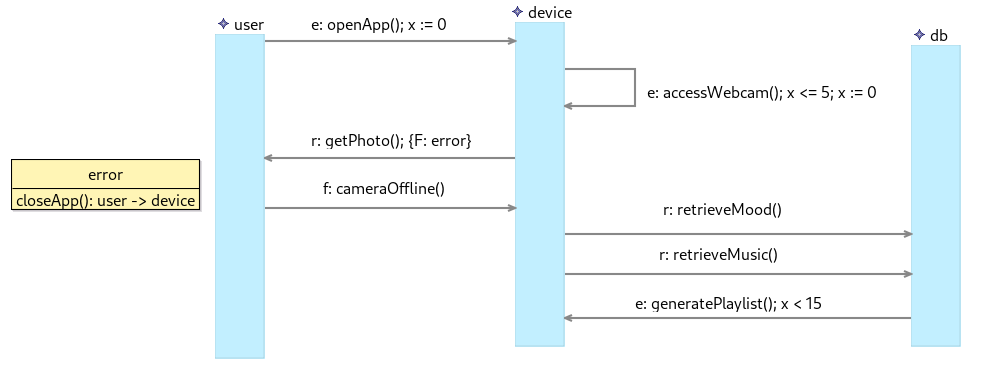
\includegraphics[width=150mm, keepaspectratio]{figures/diagramMobileExample.png}
    \caption{Második Szcenárióhoz tartozó diagram vizualizációja.}
    \label{second_visualization}
\end{figure}

A tesztrendszerünk egy zene lista generáló alkalmazás, ami egy felhasználót, mobileszközt és adatbázist tartalmaz.
A felhasználó "\textit{kedve}" alapján generálja a listát, amit az arc kifejezése alapján határoz meg.
A követelményben a rendszer alap működése van leírva egészen az elejétől, amikor a felhasználó megnyítja az alkalmazást.
A követelmény leírás megtekinthető az \ref{second_scenario_test} kódrészleten és a hozzá tartozó vizualizáció a \ref{second_visualization} ábrán.

A szcenárióhoz tartozó tesztesetek a következők:

\begin{itemize}
    \item testMobileRequirementSatisfied
    \item testMobileFutureConstraint
    \item testMobileFutureConstraintEarly
    \item testMobileWithError
    \item testMobileWithDelay
    \item testMobileWithTooMuchDelay
    \item testMobileMissingRequiredMessage
    \item testMobileRequiredEventually
    \item testMobileRequiredNotReceived
\end{itemize}

A teszteseteket a monitor hiba detektáló képeségét tesztelik.
A \textit{testMobileWithDelay} és \textit{testMobileWithTooMuchDelay} tesztesetek az \textit{x <= 5} időzítési feltétel beteljesülését ellenőrzik.
A \textit{testMobileWithDelay} 5 másodperces késleltetéssel küldjük az \textit{accessWebcam} üzenetet, míg a másiknál 6 másodperces késleltetéssel.
Az első esetben a monitornak helyes működést kell érzékelnie a következőben pedig hibás működést.

%----------------------------------------------------------------------------
\clearpage\subsection{Alt operátort tartalmazó tesztszenárió}
%----------------------------------------------------------------------------

A tesztszcenárióhoz tartozó rendszerünk egy banki rendszer.
A szcenárió megtalálható az \ref{thrid_test_scenario} kódrészleten és a hozzá tartozó vizualizáició a \ref{third_visualisation} ábrán látható.

\begin{lstlisting}[language=java, frame=single, float=ht!, caption={Alt operátort tartalmazó tesztszcenárió.},captionpos=b,,label=thrid_test_scenario]
specification Bank {

    object UserInterface ui;
    object ATM atm;
    object BankDB db;

    bool success = true;

    constraint b {
        message logout() ui->atm;
    }

    scenario transaction {
        message login(success) ui->atm;

        alt (equals(success, true)) {
            pastConstraint {b} message wReq() ui->atm;
            message uDB() atm->db;
        } (equals(success, false)) {
            message loginUnsuccessful() ui->atm;
            required message lockMachine() atm->ui;
        }
    }
}
\end{lstlisting}

\begin{figure}[!ht]
    \centering
    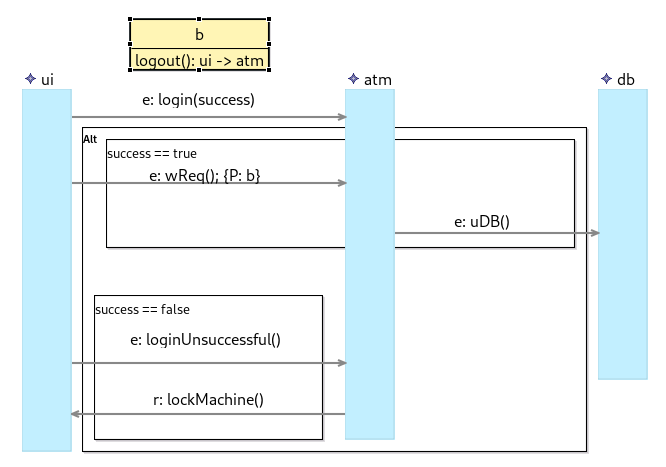
\includegraphics[width=150mm, keepaspectratio]{figures/diagramAltExample.png}
    \caption{Alt operátort tartalmazó szcenárió diagram}
    \label{third_visualisation}
\end{figure}

A rendszer egy felhasználói felületből, \textit{ATM}-ből és banki adatbázisból áll.
A követelményünkben két lehetséges működést írunk le.
A \textit{success} paraméter jelzi, hogy melyik működés a helyes.
A szcenárióhoz tartozó tesztesetek a következők:

\begin{itemize}
    \item testBankMonitorPassing
    \item testBankMonitorFailing
    \item testBankMonitorFalseCasePassing
    \item testBankMonitorFalseCaseFailing
\end{itemize}

A tesztesetekkel azt vizsgáljuk, hogy a monitor képes-e a helytelen ág lefutását hibának érzékelni és a helyes viselkedés esetén detektálni a követelmény teljesítését.

%----------------------------------------------------------------------------
\clearpage\subsection{Par operátort tartalmazó tesztszenárió}
%----------------------------------------------------------------------------

\begin{lstlisting}[language=java, frame=single, float=ht!, caption={Integrációs teszteset.},captionpos=b]
specification Email {
    object Computer computer;
    object Server server;

    constraint constraints{
        message logout() computer -> server;
    }

    scenario email {
        par {
            case checkEmail {
                message checkEmail() computer -> computer;
            }

            case newEmail {
                pastConstraint {constraints} message newEmail() computer -> server;
            }
        }
    }
}
\end{lstlisting}

\begin{figure}[!ht]
    \centering
    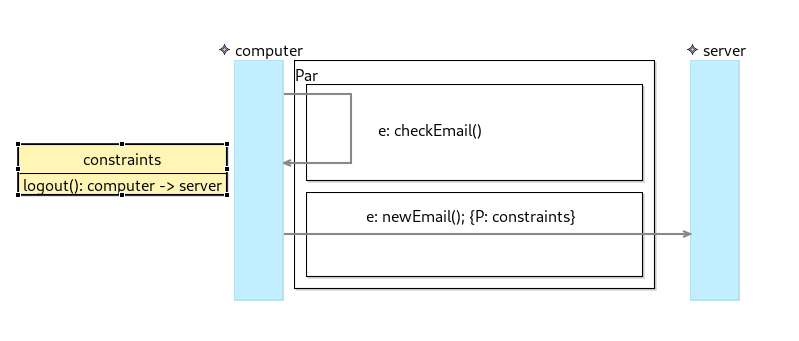
\includegraphics[width=150mm, keepaspectratio]{figures/diagramParExample.png}
    \caption{Szenárió diagram.}
\end{figure}

Ehhez a tesztszenárióhoz az első szenárióban lévő teszt rendszert használtuk fel.
A szenárióhoz tartozó tesztesetek a következők:

\begin{itemize}
    \item testNetworkRequirementSatisfied
    \item testNetworkOtherRequirementSatisfied
\end{itemize}

Azt vizsgáljuk, hogy a monitor képes mindkét permutáció esetén érzékelni a követelmény teljesítését.

%----------------------------------------------------------------------------
\clearpage\subsection{Komplex tesztszenárió loop és alt operátorokkal}
%----------------------------------------------------------------------------

\begin{lstlisting}[language=java, frame=single, float=ht!, caption={Integrációs teszteset.},captionpos=b]
specification Connection {

    object Computer computer;
    object Server server;

    string receiver = "John";
    string subject = "Next Meeting";
    bool success = false;

    clock x;
    clock y;

    constraint logout {
        message logout() computer -> server;
    }

    constraint delete {
        message deleteEmail(subject) computer -> server;
    }

    scenario authentication {
        loop (1, 3) {
            message login() computer -> computer reset x;
            pastConstraint {logout} message attemptLogin() computer -> server reset y;
        }

        alt (equals(success, true)) {
            message checkEmail() computer -> server clockConstraint {<(x, 2)};
            required futureConstraint {delete} message newEmail(receiver, subject) computer -> server reset x;
        } (equals(success, false)) {
            required message logoutUser() server -> computer clockConstraint {>(y, 3)};
            message lockComputer() server -> computer reset y;
        }
    }
}
\end{lstlisting}

\begin{figure}[!ht]
    \centering
    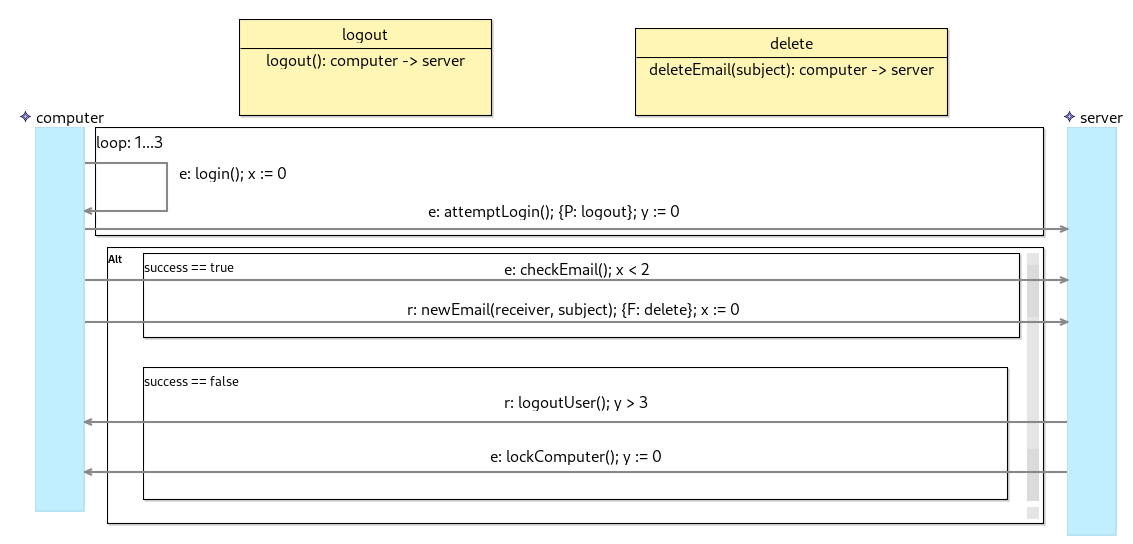
\includegraphics[width=150mm, keepaspectratio]{figures/diagramOperatorExample.png}
    \caption{Szenárió diagram.}
\end{figure}

\begin{itemize}
    \item testNetworkRequirementSatisfied
    \item testNetworkRequirementSatisfiedTwice
    \item testNetworkRequirementSatisfiedThreeTimes
    \item testNetworkRequirementSatisfiedFourTimes
    \item testNetworkAltTrueCase
    \item testNetworkAltTrueCaseSatisfied
    \item testNetworkLogoutTooFast
    \item testNetworkLogoutConstrait
\end{itemize}

\clearpage\section{Tesztelés összefoglaló}

\begin{longtable}{|p{0.1428\linewidth}|p{0.1428\linewidth}|p{0.1428\linewidth}|p{0.1428\linewidth}|p{0.1428\linewidth}|p{0.1428\linewidth}|}
\hline
\textbf{Tesztelési célok} & \textbf{Egyszerű tesztszenárió} & \textbf{Több üzenetet tartalmazó tesztszenárió} & \textbf{Alt operátort tartalmazó tesztszenárió} & \textbf{Par operátort tartalmazó tesztszenárió} & \textbf{Komplex tesztszenárió}\\
\hline
Egyszerű üzenet megjelenése & X & X & X & X & X\\
\hline
Elvárt üzenet megjelenése & X & X & X & - & X\\
\hline
Nem kivánt (fail) üzenet megjelenése & X & X & - & - & -\\
\hline
Strict üzenet tesztelése & - & X & - & - & -\\
\hline
Időzítési feltételek tesztelése & X & X & - & - & X\\
\hline
Past megkötés tesztelése & X & - & X & X & X\\
\hline
Future megkötés tesztelése & - & X & - & - & X\\
\hline
Alt operátor tesztelése & - & - & X & - & X\\
\hline
Par operátor tesztelése & - & - & - & X & -\\
\hline
Loop operátor tesztelése & - & - & - & - & X\\
\hline
Több operátort tartalmazó szenárió tesztelése & - & - & - & - & X\\
\hline
Egymást követő elvárt üzenetek & - & X & - & - & -\\
\hline
Egymást követő fail üzenetek & X & - & - & - & -\\
\hline
Sima üzenet tesztelése & X & X & X & X & X\\
\hline
Több óraváltozó & - & - & - & - & X\\
\hline
Elvárt után fail üzenet & X & - & - & - & -\\
\hline
Fail után elvárt üzenet & - & X & - & - & -\\
\hline
\caption{Összefoglaló táblázat}
\label{tab:table1}
\end{longtable}